% Use class option [extendedabs] to prepare the 1-page extended abstract.
\documentclass[extendedabs]{bmvc2k}
\usepackage[colorlinks = true,
            linkcolor = blue,
            urlcolor  = blue,
            citecolor = blue,
            anchorcolor = blue]{hyperref}
\usepackage{kotex} % 한국어 사용 가능

% Document starts here
\begin{document}
\title{Semantic Segmentation}
\addauthor{
Lee Gwan Hui$^1$, \today}{}{1}
\addinstitution{
$^1$2017142136, Department of Electrical and Electronic Engineering, Yonsei University.}
\maketitle
\let\thefootnote\relax\footnote{This is an extended abstract. The full paper is available at the \href{https://github.com/LeeGwanHui/TIL/tree/main/deeplearning_ham}{github}. }
\vspace{-0.2in}

\section{abstract}

\quad Semantic segmentation이란 pixel별로 어떤 class에 해당하는지를 찾아내는 이미지 처리의 한 분야이다. 여기서는 딥러닝을 사용해서
segmentation을 진행한 FCN 모델과 dilated convolution을 살펴볼 것이다. 

\section{FCN\cite{long2015fully}}
\quad convolutational networks은 hierarchies of features을 추출해주는 시각 모델로 기존의 이미지 처리 방법보다 성능을 현저하게 향상시켰다.
이 논문의 motivation은 classification에서 이미 높은 정확도를 가지고 있는 deeplearning models을 semantic segmentation에 사용하도록 재구조화 시키는 것이다.
Segmentation의 경우에는 pixel별로 어떤 클래스인지 파악이 되어야 하므로 input size와 같은 output size를 도출해야한다. 이 논문의 핵심을 요약하자면
convolutionalization과 up-sampling, skip-connection으로 나눌 수 있다. 
 \subsection{Introduction}
 \quad 이 논문에서 하고자 하는 것은 당시 개발된 sematic Segmentation model보다 성능이 뛰어난 model을 
 설계하는 것과 동시에 end-to-end for pixelwise prediction 과 supervised pre-training 학습이 가능하도록 하는 것이다.
 \subsection{FCN 구조 설명}
 \quad receptive field란 것은 output layer의 element하나에 영향을 미치는 input elements이다. 이를 시각적으로 내타내면 더 이해하기 쉽다. 
 이걸 먼저 설명한 이유는 이 논문에서는 patchwise training으로 사용한 것이 아니라 계산량의 효율성을 위해서라도
 겹치는 receptive field가 없도록 fully convolutional training을 사용하였다.(input image 전체를 사용) 이 논문에서는 upsampling 방법에 많은 초점을 두는데
 왜냐하면 segmentation task 상 output image가 input image와 size가 같아져야 하는데 이때 upsampling 방법에 따라 Segmentation의 정확도가 차이가 나기 때문이다.
 그래서 downsampling할 때 그 공간적 정보를 저장해서 upsampling에 사용하는 Shift-and-stitch와 계산량을 줄인 trick를 고려하지만 결국 학습형 upsampling 방법인 
 transposed convolution이 성능이 제일 좋아 사용한다. 그럼 이제 FCN의 구조를 살펴보자. 
 \newline  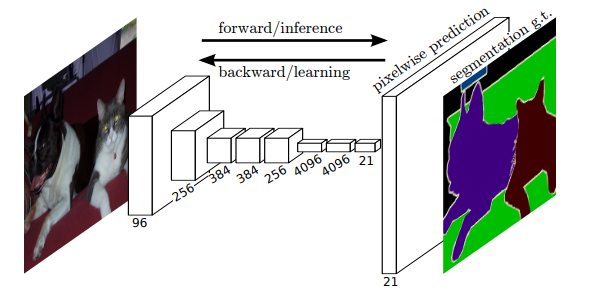
\includegraphics[width=\linewidth]{images/00_FCN.PNG}
 \quad 기존의 classification task models의 경우에는 classifier 부분이 삽입되어 있었고 vectorized 한 형태였다. 하지만 segmentation에서는 각 pixel별로 class를 예측해야하기
 때문에 각 pixel별로 class 수만큼의 channel을 가진 output이 필요하다. 그래서 마지막 단이 class의 갯수인 20개와 배경을 더해서 21개가 되는 것이다. 
 간단하게 말해서는 기존의 classification model에서 공간적 정보를 무시하고 마지막단에 사용하는 FC layer을 
 1x1 convolutational layer 형태로 바꾸어준 것으로 이로 인해 공간적인 정보를 저장하고 있을 수 있다. 그럼 이제는 FCN 모델을 통과해서 나오는 결과를 transposed conv를 통해 upsampling하는 방법이 중요하다. 
 \subsection{Skip connection 구조 설명}
 \quad skip connection을 간단하게 요약하자면 layer을 깊이 통과할수록 얻을 수 있는 hierarchies of features(coarse,semantic)과 비교적 얕은 layer의 output에서 얻을 수 있는 location, appearance information
 정보를 합쳐서 두개의 장점을 혼합하는 것이라고 할 수 있다. 자세한 구조는 아래와 같다. 
 \newline  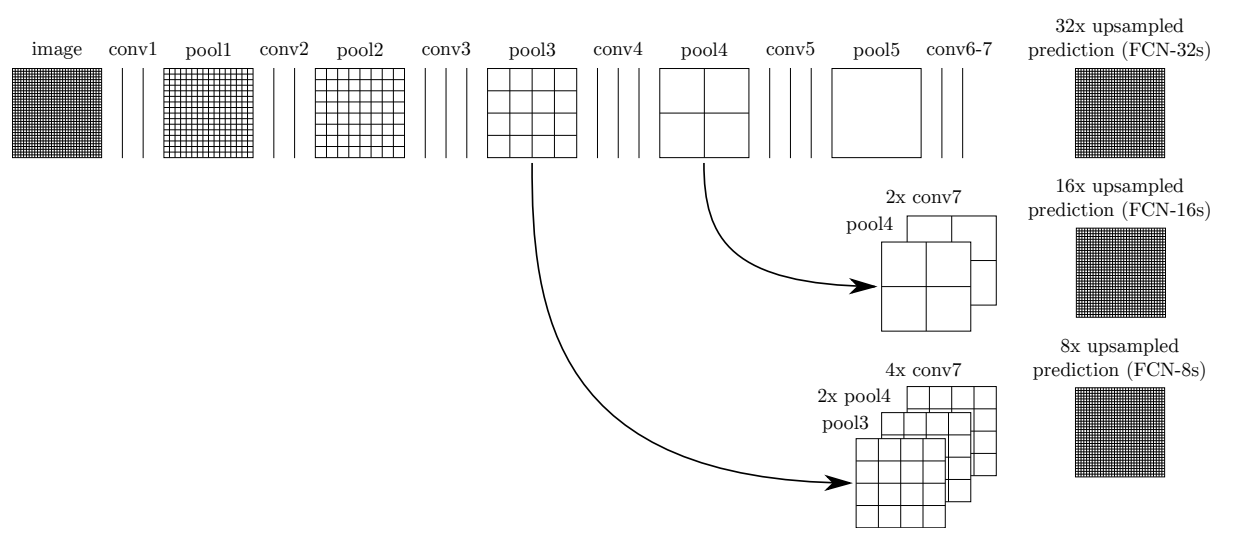
\includegraphics[width=\linewidth]{images/01_FCN.PNG}
 \quad downsampling을 하는 이유는 parameter 수를 줄여서 더 깊은 layer를 쌓기 위해서라고 볼 수 있는데 이 때 더 의미있는 features을 뽑을 수 있다는 장점이 있지만 
 localization 측면에서는 공간적 정보를 손실한다는 단점이 있다. 따라서 downsampling에서 잃어버리는 위치정보를 보안하기 위해서 고안된 것이 skip connection이다. 
 FCN-32s의 경우에는 output 1x1 matrix에서 32배 upsampling을 deconvolutional filter을 사용해서 진행한 것이다. 반면 
 FCN-16s의 경우에는 마지막 단의 1x1 matrix를 2x2 matrix가 되도록 bilinear interpolation을 진행하고 이와 pool4에서 나오는 output 결과를 더해준다.
 그 후에 16배 upsampling한 것이다.
 마지막으로 FCN-8s의 경우에는 FCN-16s와 마찬가지로 진행하되 pool3 output까지 사용한 것이다.
 \newline  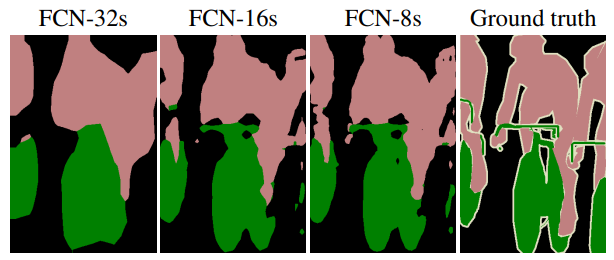
\includegraphics[width=\linewidth]{images/02_FCN.PNG}
 \quad skip connection를 채택했을 때 각 FCN에서 skip connection을 어디에서 적용해주었냐에 따라 몇가지 모델을 만들 수 있었다. 위 결과를 보면
 알수있듯이 downsampling에서 잃어버리는 location 정보를 더 얕은 layer의 output에서 고려해줄수록 segmentation 결과가 더 좋은 것을 확인할 수 있다.
 \subsection{ Results }
 \quad 추가적인 결과로는 classification model 중에서도 GoogLeNet과 VGG16은 classification 결과에서는 
 큰 차이가 없었지만 FCN을 적용할 때 segmentation에서는 큰 정확도 차이가 났고 심지어 FCN-VGG16가 더 높았다. 이 논문에서  
 SDS model과도 비교했는데 더 많은 pixel별 class의 정확도를 가지고 있고 심지어 테두리 부분도 더 매끄럽게 추출하였다.
 \newline  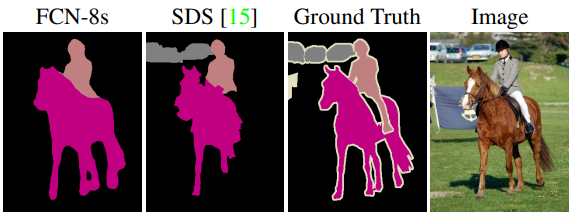
\includegraphics[width=\linewidth]{images/09_D.PNG}  

 \section{Multi-scale context aggregation by diated convolutions}
 \quad 앞선 논문에서 classification에 사용된 model을 segmentation task에 적용하는 법을 배웠는데 그 중에서도 특히 downsampling과정에서 잃어버리는 
 location 정보를 어느정도 보정하기 위해서 skip connection이 사용되었다. 이 논문에서 하고자하는 것은 downsampling에서 사용하는 pooling layer을 통해
 location 정보가 상실 된다면 아예 pooling layer을 제거하고 대체안으로 location 정보를 보존할 수 있는 sematic segmentation만을 위한 newtwork를 만들자는 것이다.

 \subsection{Introduction}
 \quad 기존에는 classification model을 사용해서 정확도를 높게 얻었지만 사실은 dense prediction과는 차이가 있다. 이 논문에서는 
 CNN model의 어떤 구조가 필요하고 없어도 되는지를 파악하여 dense prediction만을 위한 model을 설계하는 것이다. network를 간단히
 소개하면 Pooling과 subsampling 없이, convolutional layer로 구성된 rectangular 구조이다. 여기서 핵심은 dilated convolutation을 기반으로 
 설계하였다는 점이다.

 \subsection{DILATED Convolutions\cite{yu2015multi}}
 \quad 기존의 convolutional network의 구조는 아래와 같다. 
 \newline  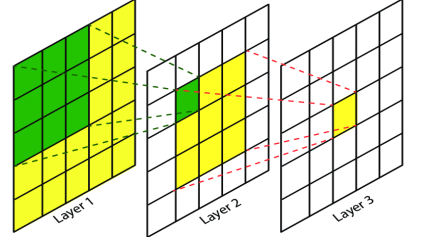
\includegraphics[width=8cm, height=3cm]{images/04_D.PNG}  
 \newline 3x3 convolutational network를 연속해서 통과시키면 receptive field가 늘어나는 것을 VGG net에서 배웠다.
 그러나 이 방법은 모서리 부분으로 갈 수록 학습이 잘 안 읽어나는 문제점과 함께 VGG net 구조상 classification을 위한 모델이기 때문에
 semantic segmentation을 적용하더라도 정확도 향상에 한계가 있다. 그래서 적용한 개념이 dilated convolution이다. 
 이는 일종의 network 경향화 기법\cite{youtube}이다.
 \newline  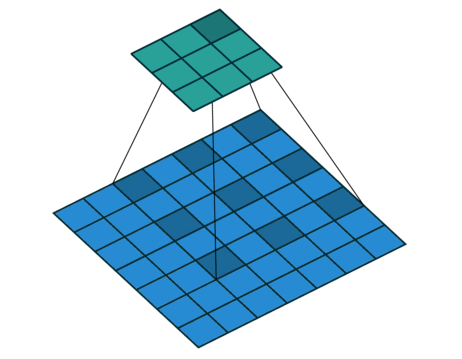
\includegraphics[width=5cm, height=3cm]{images/03_D.PNG}  
 \newline 위의 경우에는 input size가 7x7이고, kernel size는 3x3 그리고 dilation factor은 2인 경우이다.
 본래 dilation factor은 1인 경우(없는 경우)는 한 pixel이 나타내는 receptive field가 붙어있지만 dilation factor가 있는 경우에는 
 receptive field가 한칸씩 떨어져 있어서 한 pixel의 receptive field가 같은 kernel size에서 layer의 depth이 상관없이 늘어나는 것을 확인할 수 있다.
 이 방법을 사용하면 resolution이나 수렴이 늦게되는 문제없이 receptive field를 기하 급수적으로 확장할 수 있다.
 아래 그림을 보면 dilation factor라는 개념이 같은 kernel size와 같은 depth에서 얼마나 receptive field를 늘이는지 확인할 수 있다.
 \newline  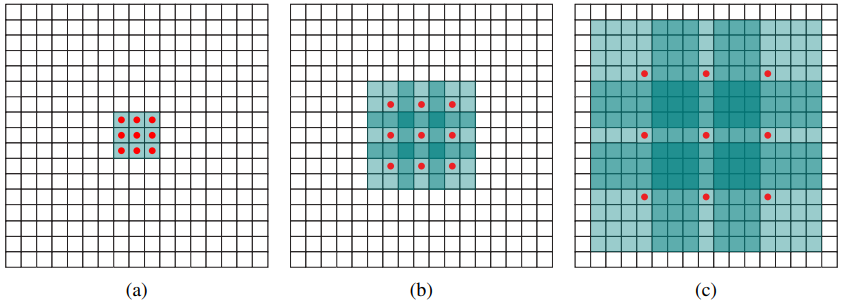
\includegraphics[width=\linewidth]{images/05_D.PNG}
 왼쪽부터 순서대로 dilation factor가 1,2,4 인 경우이다.

 \subsection{MULTI-SCALE CONTEXT AGGREGATION}
 \quad 이 논문에서는 context module을 multi-scale contextual information을 종합하여 dense prediction의 성능을 향상시키도록 설계하였다. 
 실험에서 basic모델과 좀 더 정확도를 높이기 위해 parameter을 증가시킨 large form 두가지로 만들었다. 
 \newline  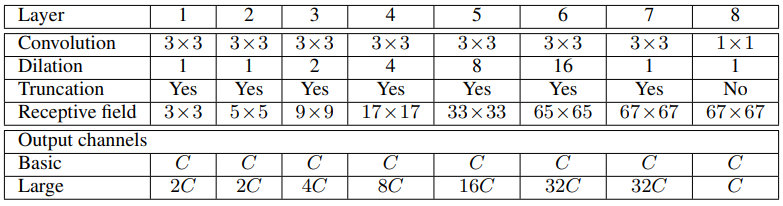
\includegraphics[width=\linewidth]{images/06_D.PNG}
 위에서 의미하는 truncation은 ReLU을 의미한다. 또한 성능향상을 위해서 initialization을 random distribution이 아닌 identity initialization을 사용하였다.
 여기서 말하는 identity initialization은 layer의 input과 동일한 output이 나오도록 초기화하는 것이다. 

 \subsection{Front-End prediction Module}
 \quad 이 논문은 VGG16 net을 수정하여 module을 설계하였는데 수정한 부분은 마지막 2개의 pooling과 striding layer를 제거하고 
 제거된 pooling layer의 역할인 downsampling을 진행하기 위해서 그 후의 layer부터는 dilation factor를 2로 설정했다.
 특히 마지막 convolution은 dilation factor를 4을 주었다. 그리고 semantic segmentation은 문맥정보가 중요하기 때문에 zero padding보다는
 reflection padding을 사용하였다.
 \newline  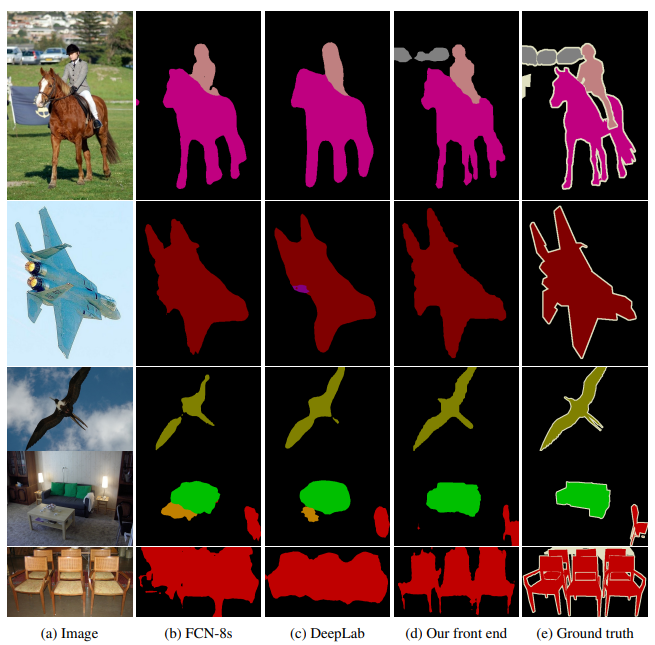
\includegraphics[width=9.5cm, height=8cm]{images/07_D.PNG}
 \newline 위의 결과를 보면 당시 나온 semantic segmentation model보다 더 세심하게 output이 검출된 것을 확인할 수 있다. 

 \subsection{failure}
 이 논문에서는 자신의 논문에서 잘 검출하지 못한 결과도 첨부하고 있다.
 \newline  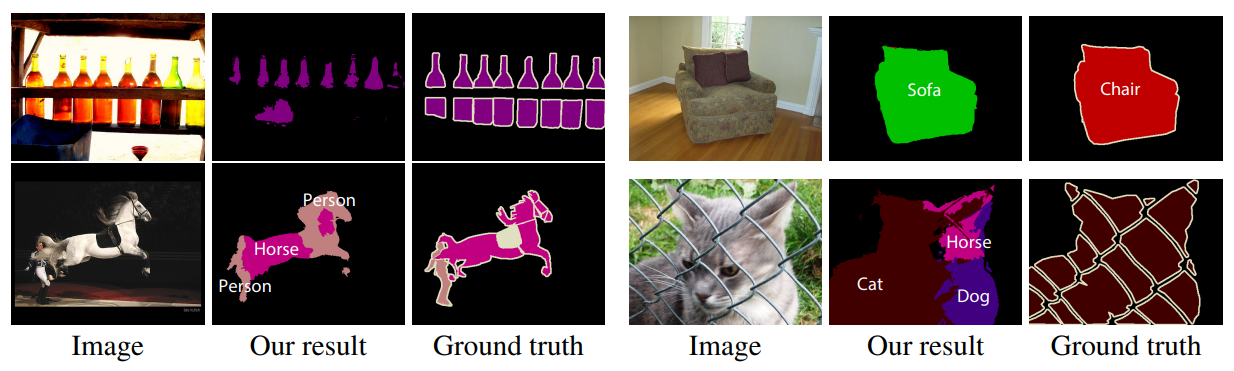
\includegraphics[width=\linewidth]{images/08_D.PNG}
 
 \section{Conclusion}
 semantic segmentation은 pixel별로 class를 예상하는 기법이다. 여기서는 deeplearning을 사용한 segmentation의 시초인 논문과 모델의 경량화 및
 더 좋은 성능을 가지게 해주는 dilated convolution을 제시한 논문을 살펴보았다. segmentation 분야는 특히 medical 분야에서 단 조금의 오차도 허용하지 않는 
 첨단 수술을 위해서 주로 개발되고 있다. 즉 output pixel의 하나하나의 정확도가 중요한 분야에 사용된다. 현재는 medical 분야에서는 Unet의 발전 모형으로 
 각 data별 pre-training을 강조한 nnUnet\cite{isensee2018nnu}이 좋은 결과를 내고 있다.

\newpage
\bibliography{egbib}

\end{document}